\documentclass{article}
\usepackage{graphicx}
\usepackage{amssymb}
\usepackage[utf8]{inputenc}
\usepackage{geometry}
\usepackage{hyperref} %Este paquete es para los URL o Links.
\geometry{left=1in, right=1in, top=1in, bottom=1in}
\title{\bfseries Collection} 
%\vspace{-1cm}; recordar este comando para dismuir la separación
\author{Alejandra Marulanda Gallego}
\begin{document}
\maketitle
\section{Tesis Valeria (Modelo molecular exacto para los estados S de los átomos de dos electrones. Aplicación al estado basal del He y de su serie isoelectrónica)}
Se introdujo una factorización exacta y única de la función propia
en términos de una amplitud marginal. Está depende funcionalmente
de la distancia interelectrónica (r12) y de una amplitud condicional,
la cual a su vez depende funcionalmente de las distancias electrón-núcleo
r1,r2 y paramétricamente de r12. Luego, se aplicó el principio variacional 
deduciendo así las ecuaciones de valor propio para las dos amplitudes.\newline
\textbf{La ecuación marginal} incluye un hamiltoniano efectivo, el cual
contiene una curva de energía potencial no adiabática que toma en cuenta 
todas las correlaciones entre las partículas de manera promediada, cuyo 
valor propio único es la energía interna. Por otro lado, en cada punto r12 
tal curva es, a su vez, el valor propio único en \textbf{la ecuación condicional}.\newline
\textbf{En conclusión}, empleando el estado basal del He y de su serie 
isoelectrónica como prototipo, se demostro que dicha curva proporciona una
interpretación de la estructura del átomo análoga a la de una molécula 
diatómica.\newline
La ecuación de Schrödinger para los sistemas atomicos conformados 
por más de un electrón no tiene solución exacta debido a las repulsiones
interelectrónicas.   
\section*{Conceptos}
\subsection*{Tesis Valeria}
\begin{itemize}
    \item \textbf{Factorización exacta:} 
    \item \textbf{Función propia:}
    \item \textbf{Amplitud marginal:}
    \item \textbf{Distancia interelectrónica:}
    \item \textbf{Amplitud condicional:}
    \item \textbf{Dependencia funcional:}
    \item \textbf{Dependencia parametrica:}
    \item \textbf{Principio variacional:}
    \item \textbf{Ecuación de valor propio:}
    \item \textbf{Ecuación marginal:}
    \item \textbf{Hamiltoniano efectivo:}
    \item \textbf{Curva de energía potencial:}
    \item \textbf{No adiabática:}
    \item \textbf{Correlaciones:}
    \item \textbf{Valor propio:}
    \item \textbf{Ecuación condicional:}
\end{itemize}
\section{Formalismo}
Coordenadas de Hylleraas:
Hylleraas mostró que la función de onda electrónica para
cualquier estado S de un átomo de dos electrones, considerando
el centro de masa el núcleo, se puede factorizar en una parte 
angular y otra interna, donde la última se puede expresar en 
términos de r1, r2 y r12. 

\begin{figure}[htb]
    \centering
    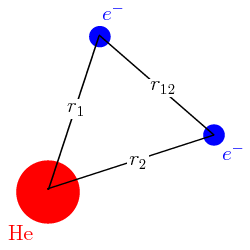
\includegraphics[width=5cm, height=5cm, scale=0.5]{modelo_de_atomo_de_helio.PNG}
    \caption{Modelo de atomo de helio.}
\end{figure}

Estas coordenadas determinan la forma y el tamaño del triángulo
electrón-núcleo-electrón y son independientes entre sí, excepto 
que deben satisfacer la desigualdad triagular:\newline

\begin{center}
\mid r12-r2\mid \leqslant r1 \leqslant r12+r2 
\end{center} \newline

Por otro lado, la función angular determina la orientación de 
dicho triángulo en el espacio. Para nuestros propósitos, no se 
necesita especificar esta función, debido a que los estados S 
tienen simetría esférica. Por lo tanto, la ecuación de Schrödinger
interna,\newline

determina la energía no relativista del átomo. En unidades 
atómicas, el Hamiltoniano radial de Hylleraas es

Se desea construir uba CEP no adiabática (CEPNA) para el grado de libertad
radial r12, lo cual se logra promediando sobre las variables r1 y r2 de la
siguiente manera. La función de distribución conjunsta está dada por


De acuerdo a la regla de Bayes, esta función se puede factorizar como


donde


Es la función de distribución marginal para encontrar a los electrones en una 
vecindad infinitesimal de r12 independientemente de (r1,r2), y Dc(r1,2|r12)
es la función de distribución condicional para encontrar a los electrones 
en una vecindad infinitesimal de (r1,r2) dado que tienen un valor determinado 
de r12. La normalización de D(r1,r2,r12),


automáticamente implica la normalización de Dm(r12),


y la normalización local de Dc(r1,2|r12),


Siguiendo a Hunter, introducimos la FMC de la función propia


donde hemos definido las amplitudes marginal y condicional como


respectivamente, de tal forma que 


Nótese que la FMC no supone una separación adiabática de los grados de libertad, es decir,
que r1 y r2 son lentos en comparación con r12. Por otro lado, la fase ..., con ... real,
es arbitraria y se escoge a conveniencia.
Las condiciones de normalización ahora quedan expresadas como 


Para obtener las ecuaciones que gobiernan a Y y X utilizamos el principio
variacional de la siquiente forma. Primero, planteamos el funcional


donde el primer término es el valor esperado de la energía, el segundo 
término asegura la normalización local de X(r1,r2|r12) en cada punto r12, y el tercer
término garantiza la normalización de Y(r12), siendo Lambda(r12) y E los
multiplicadores de Lagrange. Posteriormente, se impone la condición de extremización
dF=0, de donde se obtienen las ecuaciones


donde


En la Ecs. (18) T12, dado por la Ec.(20), se interpreta como el operador de la energía cinética
radial del movimiento relativo entre los dos electrones. En la Ec.(22) la notación ...
indica que este operador depende explícitamente de Y(r12).
Las Ecs. (18) y (19) constituyen un par de ecuaciones exactas de valores propios acopladas,
con las siguientes características. Primero, ya que los operadores son hermíticos
los valores propios E y U(r12) son reales. Segundo, al sustituir la Ec.(21) en la Ec.(18)
se obtienen qu ...Además, al manipular las ecuaciones se obtiene que también ....Por lo tanto,
.... A partir de la Ec.(19), ..., por lo que esta función contiene toda la información sobre
las atracciones electrón-núcleo, la repulsión interelectrónica y el acople cinético,
promediados sobre r1 y r2. Así, en la Ec.(18) U(r12) juega el rol de un potencial efectivo
que, sin embargo, correlaciona los electrones completamente; ésta es nuestra CEPNA atómica. 

Los electrones están correlaciones, no solo por las repulsiones electrostáticas
(correlación de Coulomb)sino también por las fuerzas de intercambio (correlación de
Pauli). La correlación de Paulo se puede incluir exactamente utilizando
un producto antisimetrizado de espín-orbitales (determinantes de Slater). La
correlación de Coulomb se puede incluir aproximadamente por medio de la teoría de 
perturbaciones de Moller-Plesset o de expansiones multiconfiguracionales, como 
la interacción de configuraciones y los cúmulos acoplados. 
EN el marco de mecánica cuántica, la noción de que las moléculas poseen una 
estructura bien definida se basa en la topografía de la superficie de energía
potencial (SPE), obtenida mediante la aproximación Born-Oppenheimer (ABO), donde
las estructuras de equilibrio se definen a partir de los mínimos locales de la SEP.
No obstante, la ABO solo aplica a sistemas que permiten una separación adiabática 
de los grados de libertad (asume que el moviemineto electónico y nuclear se pueden
desacoplar).
OBJETIVO: Extender el concepto de SEP a cualquier sistema de partículas, ya que sería
muy conveniente desde el punto de vista conceptual e interpretatico, pues permitiría 
conservar la idea de una estructura geométrica y crear un tratamiento unificado para 
diferentes tipos de sistemas. 
EL primer paso fue dado por Feagin y Briggs ("Métodode orbitales moleculares" para la 
descripción de los estados doblemente excitados de He, empleando la distancia 
interelectrónica,r12, como una coordenada adiabática análoga a la distancia 
interprotónica, R, en el H2+), pero este modelo es aplicable solo a 
estados doblemente excitados, donde la separación abiabática de los grados de libertad
es factible. 
El profesor Arce y Laura demostraron la posibilidad de generalizar el concepto de SEP a 
estados que no permiten una separación adiabática de grados de libertad, utilizando una
factorización marginal-condicional (FMC) exacta de la función de onda. Mostraron que es 
posible obtener una SEP no adiabática radial, U(r1,r2), para estados S de dos electrones, 
definiendo la amplitud marginal como una función de las distancias electró-núcleo, r1,r2,
y la amplitud condicional como una función de la distancia interelectrónica, r12, dependiendo 
paramétricamente de r1,r2. Esto se aplicó al estado basal del He, empleando funciones de 
onda explícitamente correlaciones tipo Hylleraas, lo cual permitió realizar una interpretación
tipo molecular de los movimientos radiales de los electrones y del papel de las correlaciones
Coulombiana y cinética. 
En el caso de Valeria, se introdujo una FMC donde la amplitud marginal y condicional eran 
inversas a las seleccionadas por el profesor Arce y Laura. Como prototipo, se aplico este método
al estado basal del He y de su serie isoelectrónica. Complementando con lo que ya estaba, esto 
permitió asignarle una estructura geométrica al átomo, y determinar los efectos sobre ella 
de las correlaciones Coulombiana y cinética. 
\begin{center}

\end{center}

\end{document}
